\subsection{Project Jupyter}
\label{sec:project-jupyter}

% Figure has been moved into concept.tex. Label remains the same.
% \begin{figure}[htb]\centering
%   \includegraphics[width=0.9\textwidth]{use-cases-binder-logbook-solution.png}
%   \caption{A typical use case for Jupyter notebooks in research.
%             Image by Juliette Belin for the OpenDreamKit project, used under
%             CC-BY-SA.}\label{fig:use-cases-binder}
% \end{figure}

\subsubsection{Relationship between the \TheProject{} project and the Jupyter ecosystem}

Some of the team member of the proposed SOURCE project have a track record as
developers and contributors to Project Jupyter and its associated
ecosystem, including Jupyter Notebook.

The proposed work will improve the reproducibility of research that uses
notebooks, but it is a key aspect of the proposal to make the potential
impact of the Binder tools for reproducibility available to those researchers
who have no desire or possibility to use notebooks in their work.

In this section, we introduce key components of project Jupyter to help
contextualise the Binder project that is described subsequently, and the focus
of the proposed work.


% \TheProject has chosen to centre its efforts on the Jupyter software
% ecosystem, in particular Binder and repo2docker.
% Figure~\ref{fig:use-cases-binder} summarises a typical use
% case of Jupyter Notebook and Binder;
% both are described in more detail below.


\subsubsection{Project Jupyter}\label{seq:project-jupyter-number-notebooks}

\emph{Project Jupyter} \cite{Jupyter}, which has grown increasingly popular in the scientific
computing community, has become the \emph{lingua franca} of interactive
computing in both academia and industry \cite{Perkel2018}. The main goal of Project Jupyter
is to provide a consistent set of tools to improve researchers'
workflows from the exploratory phase of the analysis to the communication
of the results \cite{Kluyver2016,Granger2021}.

Split in 2014 from the \emph{IPython Project} \cite{IPython}, Jupyter has grown
rapidly in popularity and adoption both in the industry and academia. We
estimate the user base of the Jupyter notebook to be in the millions
\cite{jupyter-grant}. Users range from data scientists to researchers,
educators, and students from many fields, including journalists and librarians.
The number of publicly hosted Notebook documents is exceeding 8~millions~\cite{notebookcount}.

%%% The award is mentioned in the 'excellence' section in 1.1 now. No need to
%%% repeat I would say.
%
% In 2017, the Jupyter team was awarded the \emph{ACM Software System Award}, an
% annual award that honors people or an organization \emph{"for developing a
%   software system that had a lasting influence"}. Prior recipients include
% \emph{Unix}, \emph{TCP/IP}, and the \emph{World Wide Web} \cite{acm-award}.

A large number of discrete software components make up Project Jupyter.
While these interact with one another, many can be installed separately
to serve various use cases.

% For this proposal, we loosely divide the
% software involved into \emph{Jupyter core} developed under the guidance
% of the developers who started the project, and the broader \emph{Jupyter
% ecosystem} including software developed by third parties,
% which may interact or build upon core Jupyter components.

Some of the components and concepts important to \TheProject are detailed below.

\begin{figure}[ht]\centering
  \centering
  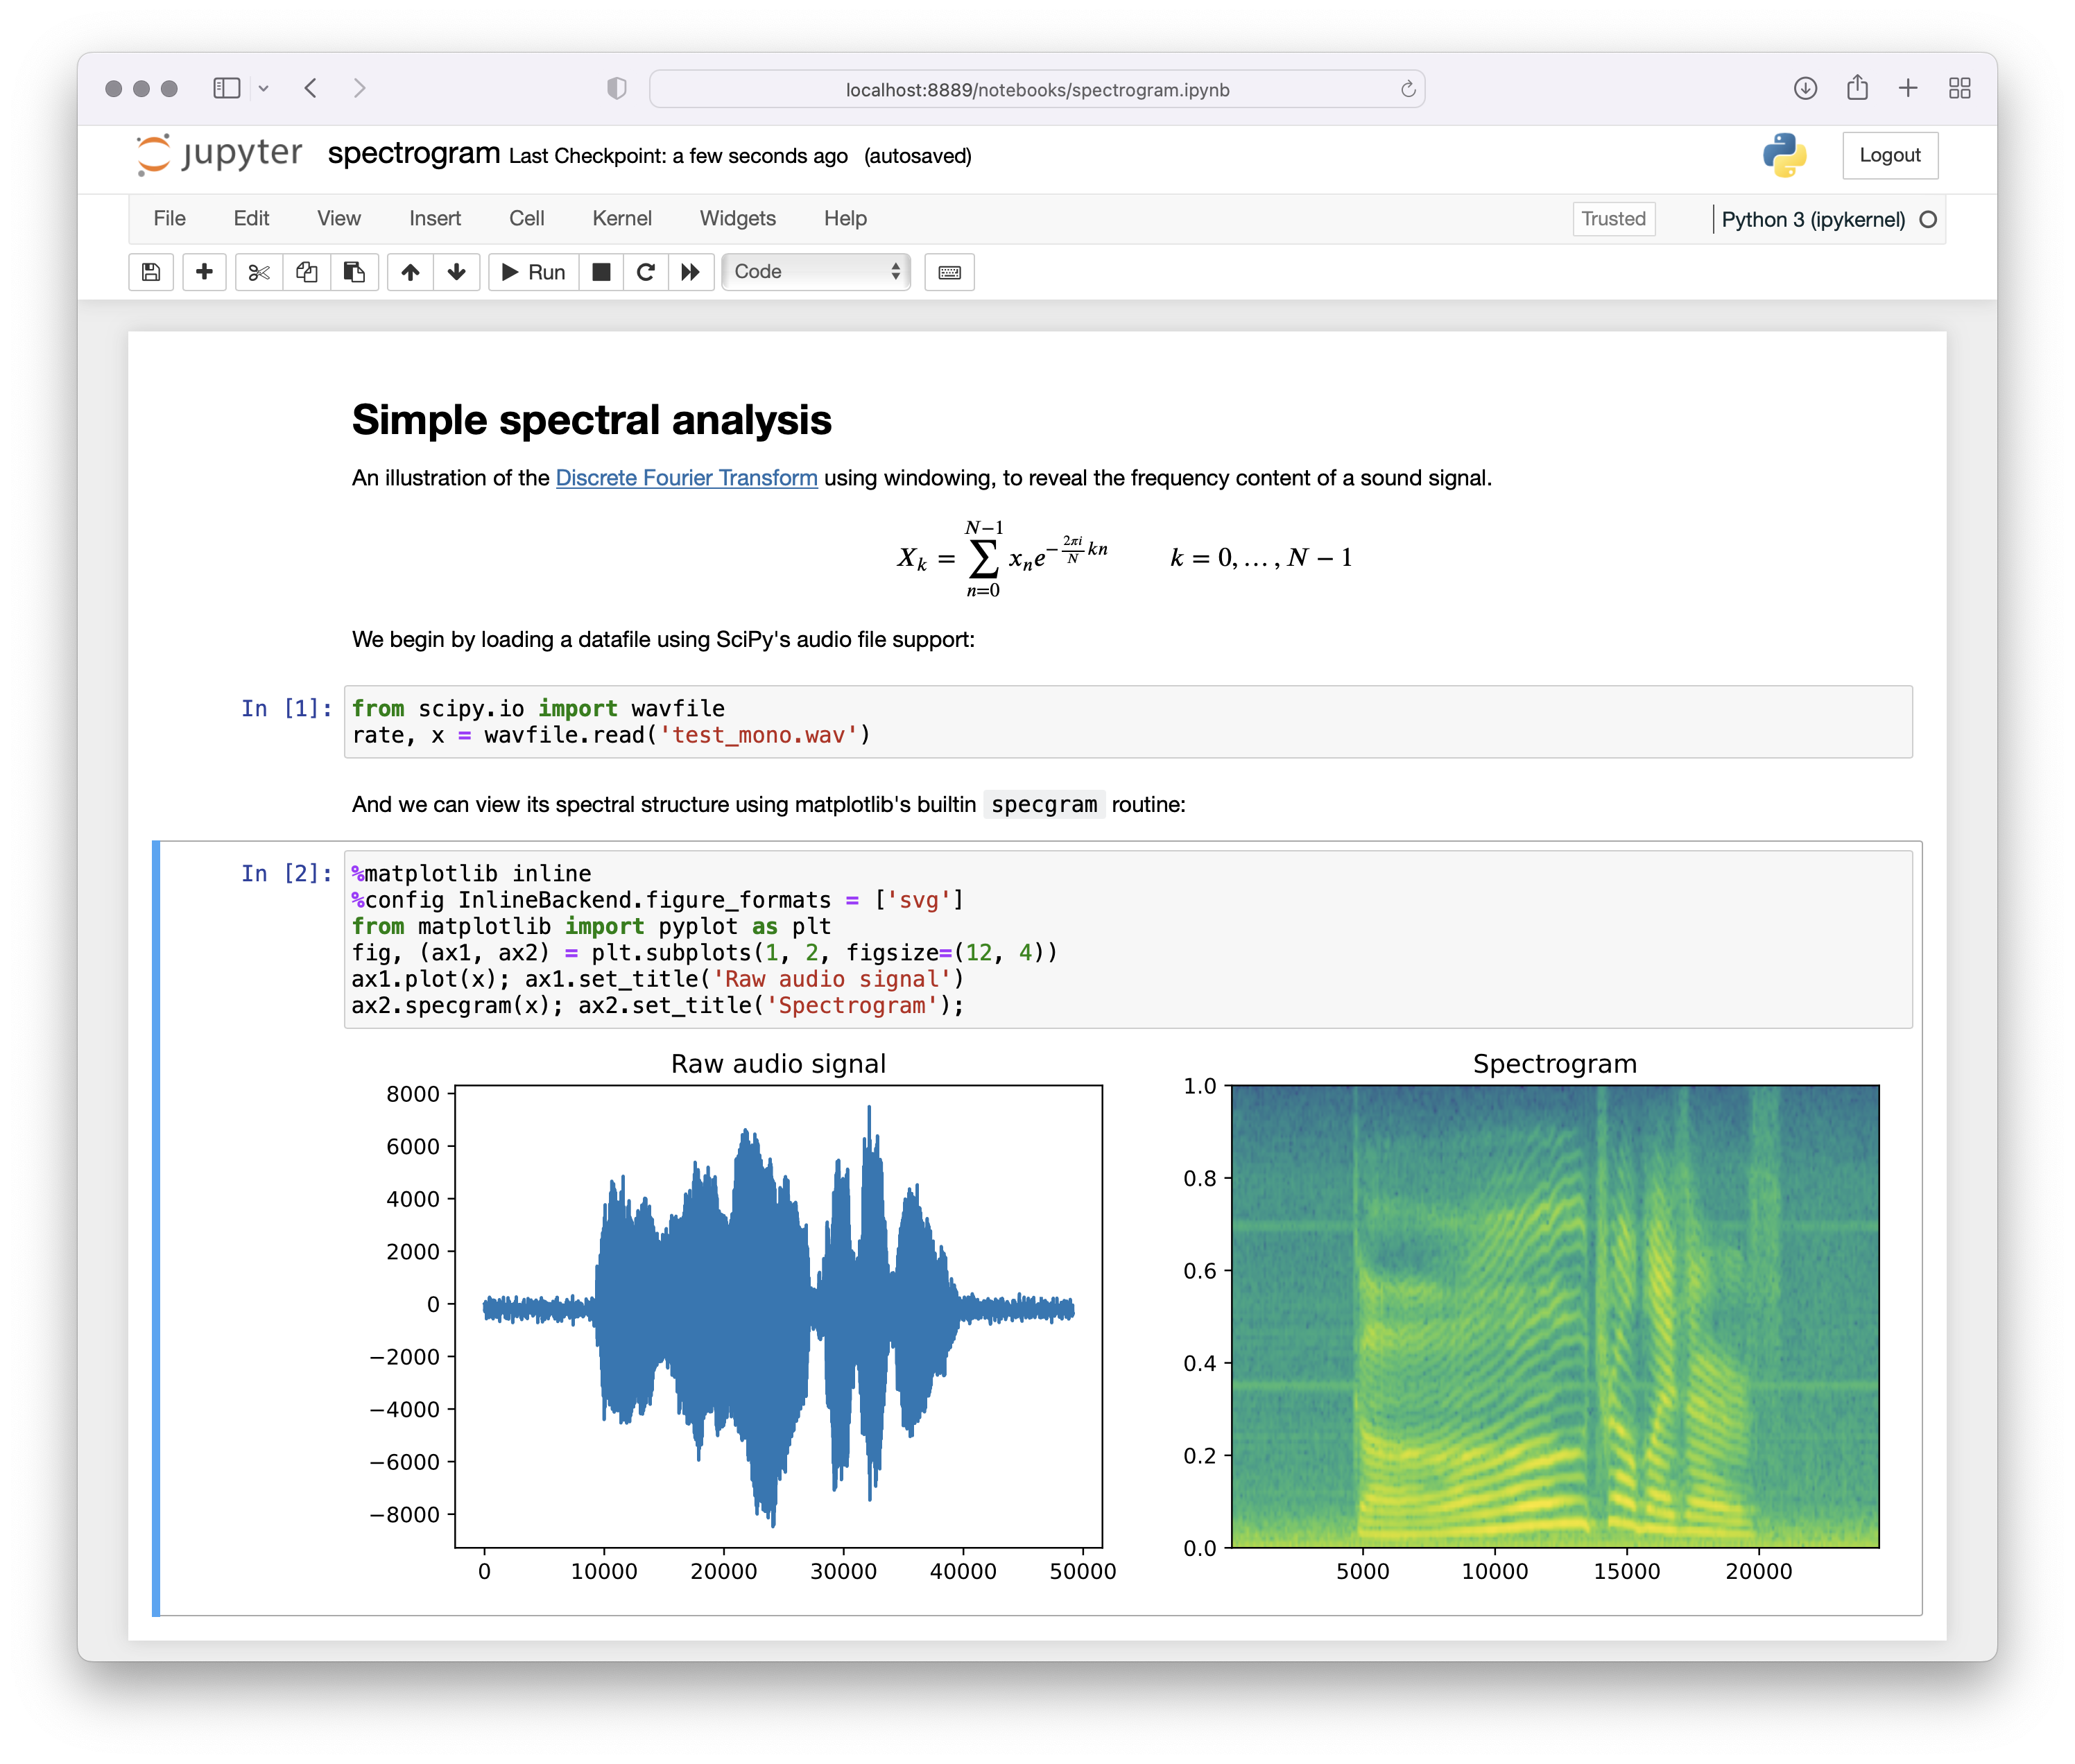
\includegraphics[width=0.9\textwidth]{images/spectrogram.png}
  \caption{A notebook document in the Jupyter Notebook interface.}\label{fig:notebook-screenshot}
\end{figure}

\subsubsection{Jupyter Notebook}\label{sec:jupyter-notebook} The Jupyter Notebook is
the flagship application of Project Jupyter. 
It allows the creation of notebook documents, containing a mixture of text and
interactively executable code, along with rich output from running that code.
Figure \ref{fig:notebook-screenshot} shows an open notebook including graphs
from an audio processing example. Notebook documents are readily shareable,
providing a popular way to describe and illustrate computational methods and
tools. \TODO{We should update the notebook: (i) point to a github repo with it,
  and (ii) binder-enable it. Sources are in data/notebook-figure} \textbf{Jupyter Lab} is the new, modular, extensible
client application for Jupyter notebooks, but the document format, server, and
user model are the same.

\subsubsection{JupyterHub}\label{sec:jupyterhub} JupyterHub is a multi-user extension of the Jupyter Notebook.
It runs on one or more notebook servers, for example at a research institution.
Users can log in to author and run notebooks through their web browser, without
needing to install any software on their own computer (because the research
software that is executed is located with the JupyterHub installation at the
research institution).

The communication between the notebook server (for example at the research
institution) and the client (for example the researcher with their laptop in the
home office) is based on the standard https protocol, and the connection is
efficient. The researcher -- as the client of the connection to the JupyterHub --
only needs a web browser, and very modest hardware to be able to access
supercomputers or cloud resources remotely.

\TODO{Add an image with a schematic of JupyterHub here?}

Because of these characteristics, many research institutions and HPC centres host their own
JupyterHub service to provide access to large compute resources and data hosting
hardware. Users of the service can connect remotely and conduct computational
exploration or data analysis through the notebook interface displayed in their
web browser~\cite{Fangohr2020}.
%% Some of this detail is now in the ambition section.
% 
% JupyterHub installations are also seen as important
% for EOSC, for example~\cite{panosc-jupyter-binder}. \TODO{Would be good to list
%   one or two more EOSC projects / activities / EGI JupyterHub link}


% \medskip\noindent\emph{Jupyter ecosystem}\label{jupyter-ecosystem}
% 
% While Jupyter is a large, distributed, coordinated project,
% the wider community of Jupyter users develops a great deal of
% software with Jupyter integration,
% providing increased or domain-specific functionality,
% building on top of Jupyter, or integrating core Jupyter components in some aspect.
% We call this the \textbf{Jupyter ecosystem}.
% The broader Jupyter ecosystem includes many more projects than we will describe
% here, but a selection of projects which are relevant to
% \TheProject includes:
% 
% \begin{itemize}
%   \item \textbf{Binder} builds on JupyterHub to allow sharing executable
%   environments along with data files and a description of the software components
%   required to run the notebooks. When someone accesses a Binder repository,
%   the service builds the computational environment on demand, allowing them to
%   execute and modify a copy of the notebooks.
%   \textbf{repo2docker} \cite{repo2docker} and \textbf{BinderHub} \cite{binder} are components of the Binder
%   software. \TOWRITE{}{More here, as repo2docker is key}
% \end{itemize}

% \begin{figure}[ht]\centering
%   \includegraphics[width=0.5\textwidth]{ipywidgets_example.png}
%   \caption{An example of using two simple slider widgets to explore the
%   parameter space of a function. The \texttt{@interact} decorator creates
%   the widgets and connects them to the function.}
%   \label{fig:ipywidgets-example}
% \end{figure}

\subsubsection{Jupyter notebook and reproducibility}

While Jupyter notebooks can make computational and data-driven research more effective
\cite{Perkel2018,Fangohr2020,Granger2021}, they also have great potential to push
open and reproducible science forward \cite{Beg2021}. The notebook provides a complete
description of a computational and data science study (Step 1 in
figure~\ref{fig:use-cases-binder}), and the notebook can -- in principle -- be
turned into a publication, or can be used to provide the required computation
for a part of a publication, such as a figure (Step 2 in
figure~\ref{fig:use-cases-binder}). Once the researcher has specified what
software is required to execute the notebook (Step 3 in
figure~\ref{fig:use-cases-binder}), the study is completely reproducible by
anyone (Step 4 in figure~\ref{fig:use-cases-binder}).

In this way, the notebook \emph{enables reproducibility} of complex workflows
with minimal additional effort on the user side. This approach is used by a
substantial number of scientists for publications already (for example
\cite{GitHubRepoExampleAlbert2016,GitHubRepoExampleCortes2018,Beg2019-blochpoint-data-repository, }
\TODO{insert publications with reproducible repositories - the LIGO paper?
  Anything else}): it is hard to prove
but it seems plausible that a significant fraction of the 30,000 sessions
triggered on the mybinder.org service every day are used for reproducible repositories
(Section~\ref{sec:mybinder}).

% HF: this is a reference to the Joel Grus criticism. Not sure if we need it.
% The paper by Beg2021 addresses that in section 9.
(We note in passing that the use of Jupyter notebooks alone does not guarantee
reproducibility: it requires some training and/or experience to be able to specify a
computational environment and to capture that information in a machine readable
way. It is also important to include all computational steps in the notebook in
order~\cite{Beg2021}.)


The Binder tools (Section~\ref{seq:project-binder}) were designed to execute
such notebooks in tailored computational environments which can be created
automatically and on demand (Step 4 in figure~\ref{fig:use-cases-binder}).

The fully-automated creation of the correct software environment is an
essential aspect of reproducibility that is not widely addressed yet. The
\TheProject{} project will address this need, improve the automatic software creation support
for notebook-driven computational research, and make the same improved automatic
software creation support accessible for uses cases without notebooks.

%%% Local Variables:
%%% mode: latex
%%% TeX-master: "proposal"
%%% End:
